\section{Conclusion}

\begin{frame}{Summary}
  \begin{itemize}
    \item Search Algorithms will check every possible answer in a problem, until they find the solution;
    \item The set of "every possible answer" ({\bf the search space}) depends on the data structure, algorithm, and smart pruning;
    \item The time performance of Search Algorithms depends on the size of the search space;
    \item {\bf Complete Search} takes a lot of time, but it will always find the correct answer (if the search space contains it);
    \item {\bf Binary Search} and {\bf Greedy Search} are much faster, because they discard a large part of the search space. They require special conditions for the problem;
  \end{itemize}
\end{frame}

\subsection{Search Algorithms in Research}
%% TODO: Improve the Search Algorithms in CS research ... Next time!

\begin{frame}
  \frametitle{Search Algorithms in CS Research}

  Search algortihms (including Greedy and Binary search) sound simple, but they have a very important place in CS research.\bigskip

  The key idea of search algorithms is central to the definition of NP-completeness: a solution to an NP-complete problem can be {\bf checked} in polynomial time. This implies that the approach to solve many NP-Complete problems is to define the search space, and systematically check the answers in this space: Just what we're doing!\bigskip

  This also to other problems where we do not have complete information, and/or we do not know efficient algorithms.\bigskip

  There are, of course, more complex approaches to search algorithms:
  \begin{itemize}
    \item Heuristic Search;
    \item Meta-heuristic Search;
  \end{itemize}
\end{frame}

\begin{frame}{Heuristic Search}
  {\bf Heuristic Search} is a search algorithm guided by a {\bf Heuristic function}, which is a function that {\bf estimates} the distance of an answer to the optimal solution.\bigskip

  One famous example of a heuristic algorithm is A* search, which is often used in path-finding and game AI.

  \[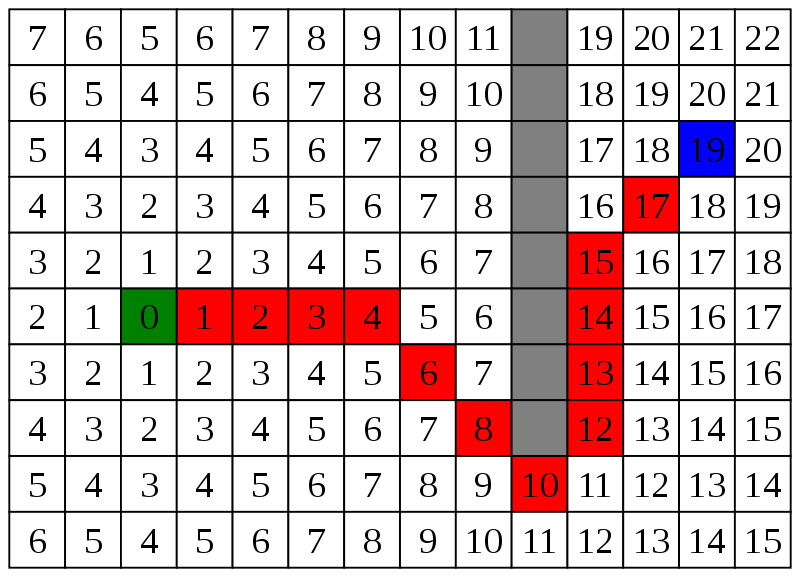
\includegraphics[width=.45\textwidth]{../img/wikipedia_pathfinding_astar}\]
  \ppagenote{A* pathing image by dbenzhuser, CC-BY-SA 2.5}
\end{frame}

\begin{frame}
  \frametitle{Meta-heuristic Search}
  Meta-heuristic search are a more general form of heuristic search. While a Heuristic search uses a function that guides the search for {\bf one specific problem}, Meta-heuristic search guides the search towards an {\bf entire category of search spaces}.\bigskip

  Meta-heuristic search are used in real world industrial optimization problems, and are an active area of research.\bigskip

  Some examples of meta-heuristics:
  \begin{itemize}
    \item Evolutionary Algorithms / Genetic Algorithms;
    \item Hill Climbing;
    \item Swarm Algorithms;
    \item Etc...
  \end{itemize}
\end{frame}

\subsection{Problem Discussion}
\begin{frame}{Problem Discussion}

  \[Finally, let's quickly overview the problems for this week: \]
\end{frame}


\begin{frame}
\frametitle{1- Dragon of Loowater}
  A dragon with many heads is attacking the kingdom, and the king is wants to hire knights to slay the dragon.
  \begin{itemize}
    \item You need one knight per head;
    \item A knight can only defeat the head if he is bigger than the head;
    \item A knight charges a reward equals to his size;
  \end{itemize}

  \begin{block}{Input}
    \begin{itemize}
      \item List of Dragon heads and their sizes
      \item List of Knights and their sizes
    \end{itemize}
  \end{block}

  \begin{exampleblock}{Output}
    \begin{itemize}
      \item Find the minimum cost necessary to defeat the dragon;
      \item Or write if it is impossible to defeat the dragon;
    \end{itemize}
  \end{exampleblock}

  {\bf Hint:} Data pre-processing is important here.
\end{frame}

\begin{frame}
  \frametitle{2- Stern-Brocot Number}
  This problem describes a tree-structure that can generate all fractions of rational numbers. For any given fraction, you must find the path in this tree that leads to that fraction.\bigskip

  \begin{block}{Input}
    \begin{itemize}
    \item Two numbers that make a fraction. e.g.: 5, 7;
    \end{itemize}
  \end{block}

  \begin{exampleblock}{Output}
    \begin{itemize}
      The path to that fraction in the tree;
    \end{itemize}
  \end{exampleblock}

  {\bf Hint}: Try to do it by hand a few times!
\end{frame}

\begin{frame}
  \frametitle{3- Bars}

  This is just the famous {\bf knapsack problem}.

  \begin{block}{Input}
    Size of the knapsack, and size of the items.
  \end{block}
  \begin{exampleblock}{Output}
    "YES" if you can solve the knapsack, "NO" if you can't.
  \end{exampleblock}

  {\bf Hint:} The knapsack problem is a permutation problem, so pruning is important! (every item you prune, the search space is cut in half)\\
\end{frame}

\begin{frame}
  \frametitle{4- Rat Attack}
    \begin{block}{}
      \begin{itemize}
      \item You have an $n\times n$ matrix (max 1024) with some rats in each cell;
      \item You have a rat trap (bomb) that kills all rats in a matrix $2d+1 \times 2d+1$
      \item Where can you put the trap to kill the largest number of rats?
      \end{itemize}
    \end{block}\bigskip

    {\bf Hint:} Search all positions for the trap, and counting all the rats at that position will take too much time. But you can change the data structure to reduce this time.
\end{frame}

\begin{frame}
  \frametitle{5- Simple Equations}

  \begin{block}{}
    Given the numbers $A, B, C$, you need to find $x, y, z$ that complete the following equations:
    \begin{itemize}
      \item $x + y + z = A$
      \item $xyz = B$
      \item $x^2 + y^2 + z^2 = C$
    \end{itemize}
  \end{block}

  {\bf Hint:} You need to search all values of $x,y,z$ (triple loop). Pruning is important;\\
  {\bf Hint:} What are the maximum and minimum values of $x,y,z$? Equation "C" is a good place to start.
\end{frame}

\begin{frame}
  \frametitle{6- Through the Desert}
  {\small
    \begin{block}{}
      \begin{itemize}
      \item Simulate a car going through the desert;
      \item Find the least amount of starting fuel needed to win.
      \end{itemize}
    \end{block}

    \begin{itemize}
    \item You could try to calculate the amount of fuel needed in each
      section of the trip (between gas stations);
    \item Or you could just simulate the trip, and make a binary
      search based on the amount of fuel left;
    \end{itemize}
  }
\end{frame}

\begin{frame}
  \frametitle{7- Zones}
  A cellphone company has a plan for $N$ towers, but will only build $M$ of them. ($M \leq N$). You know how many people are served by each tower, and you have to choose the towers that {\bf maximize} the number of people.\bigskip

  {\bf Hint:} This is a "select the maximum" subset problem. Can it be solved by greedy seach?\\
  {\bf Hint:} One big problem is the overlap between the towers. Be careful!
\end{frame}

\begin{frame}
  \frametitle{8- Little Bishops}

  \begin{itemize}
    \item Like 8 queens, but with bishops!
    \item The number of bishops and the size of the board can be very big. Be careful of TLE!
  \end{itemize}
\end{frame}
